\documentclass[letterpaper,12pt]{article}
\usepackage{tabularx} % extra features for tabular environment
\usepackage{amsmath}  % improve math presentation
\usepackage{graphicx} % takes care of graphic including machinery
\usepackage[margin=0.95in,letterpaper]{geometry} % decreases margins
\usepackage{cite} % takes care of citations
\usepackage[titletoc,title]{appendix} % takes care of appendices
\usepackage{listings} % code representation
\usepackage{pdflscape}
\usepackage{csquotes} % for quoting existing work
\usepackage{color} % defines colors for code listings
\usepackage{comment} % allows for block of comments
\usepackage{gensymb} % degree symbol
\usepackage{pdfpages} % include pdfs in the document (used for console output)
\usepackage[final]{hyperref} % adds hyper links inside the generated pdf file

% style code listings
\definecolor{codegreen}{rgb}{0,0.6,0}
\definecolor{codegray}{rgb}{0.5,0.5,0.5}
\definecolor{backcolour}{rgb}{0.95,0.95,0.92}
\lstdefinestyle{mystyle}{
    backgroundcolor=\color{backcolour},   
    commentstyle=\color{codegreen},
    keywordstyle=\color{blue},
    numberstyle=\tiny\color{codegray},
    basicstyle=\footnotesize,
    breakatwhitespace=false,         
    breaklines=true,                 
    captionpos=b,                    
    keepspaces=true,                 
    numbers=left,                    
    numbersep=5pt,                  
    showspaces=false,                
    showstringspaces=false,
    showtabs=false,                  
    tabsize=4
}
\lstset{style=mystyle}

\begin{document}

\title{IS5103 Web Technologies\\Assignment 1 Report}
\author{Student ID: 150014151}
\date{30th October, 2019}
\maketitle
\newpage

\tableofcontents
\newpage

% ---------------------------------------------------------------------------

\section{Prior Planning and Research}
\label{sec:prior-planning-research}

The first step consisted in deciding which area to present on the website: the ``Role of Web Standards'' subject was elected. Next, content about the subject was researched in order to come up with a 6-part plan. The initial draft can be found in Appendix \ref{sec:appendix-prior-initial-draft}. No content from the lecture slides was used, the references were found entirely through online searching to find interesting sources. The references used can be found directly on the website: \url{https://agj6.host.cs.st-andrews.ac.uk/references.html}. The entire content of the website, including titles, paragraphs, citations, figures and references, were typed out in a Word document like an essay (see Appendix \ref{sec:appendix-prior-planning-research-essay}), before being transformed into a web page, which is discussed in Section \ref{sec:design-content-initial-markup}.

% ---------------------------------------------------------------------------

\section{Aims of the Website}
\label{sec:aims}

The website aims to instruct the reader about the goal of having web standards and how they have affected the World Wide Web up until today. The objective is also to educate the reader about how these web standards evolved to regulate web technologies, compatibility and accessibility across of the World Wide Web, what are web standards organisations and who are the main ones, how new web standards are developed, and an overview of the most popular web standards.

% ---------------------------------------------------------------------------

\section{Target Audience}
\label{sec:target-audience}

The target audience for this website could potentially include any reader curious about how the web functions. This includes anyone interested in discovering how the web pages they visit daily are regulated, whether they have no experience in web development or are upcoming web developers who wish to extend their knowledge about web technologies.

% ---------------------------------------------------------------------------

\section{Tools Used}
\label{sec:tools-used}

The following tools were used when designing the website:
\begin{itemize}
    \item WebStorm: an IDE developed by JetBrains \cite{webstorm} to write the HTML, CSS and JavaScript code.
    \item GitHub Version Control: to backup and version the code.
    \item Google Chrome web browser: to view display the website and debug using the developer tools.
    \item Overleaf: to write the report in \LaTeX.
\end{itemize}

% ---------------------------------------------------------------------------

\section{Design and Content}
\label{sec:design-content}

The website was implemented in different iterations, starting with basic HTML markup before organising the content into different pages with navigation, followed by styling the markup and adding advanced styling features through CSS and JavaScript, and finally ending with making the website responsive and optimising imports. 

\subsection{Initial Markup}
\label{sec:design-content-initial-markup}

The first step consisted in creating an empty \textit{index.html} file in the root directory, including the metadata and an empty body before pasting the content from the Word document mentioned in Section \ref{sec:prior-planning-research}. HTML markup was then used to separate the text into headings (\textit{\textless h1\textgreater} for page title, \textit{\textless h2\textgreater} for section titles, \textit{\textless h3\textgreater} for subsection titles), paragraphs and lists. Next, markup such as anchor tags for links, figures (which include an image and a caption) and quotes was added. Once the basic markup was completed, links between the different sections of the website were created, such links from the content citations to their references, links pointing to figures and related sections.

\subsection{Website Organisation}

The second step involved separating the content into different pages. Dense content was favoured over sparse content, leading to the website being divided into three separate pages:
\begin{itemize}
    \item Home page in the \textit{``index.html''} file.
    \item Content page in the \textit{``content.html''} file.
    \item References page in the \textit{``references.html''} file.
\end{itemize}
This approach was chosen in order to avoid having multiple sparse pages with one only subtopic per page.\\

To link those pages, a header, a navbar\footnote{Navigation Bar} and a footer were added as well. The header contains the title of the website, which returns the user to the home page when clicked. The navbar is made up of links that act as buttons linking all the pages together. Finally, the footer is used for credits, but is also used to provide the user with a site map\footnote{A list of all the publicly accessible pages on a web site.} and contact information on larger websites. These three elements, along with the metadata, are the only duplicated elements across all HTML files.\\

The root directory itself is organised as follows (see Figure \ref{fig:root-structure} for more detail):
\begin{itemize}
    \item \textit{``root''}: contains the HTML files and the directories mentioned below.
    \item \textit{``images''}: contains all the images used across the website.
    \item \textit{``css''}: contains the stylesheets and the fonts.
    \item \textit{``scripts''}: contains the JavaScript functions called when an event is triggered in the HTML code.
\end{itemize}

\begin{figure}[h] 
\centerline{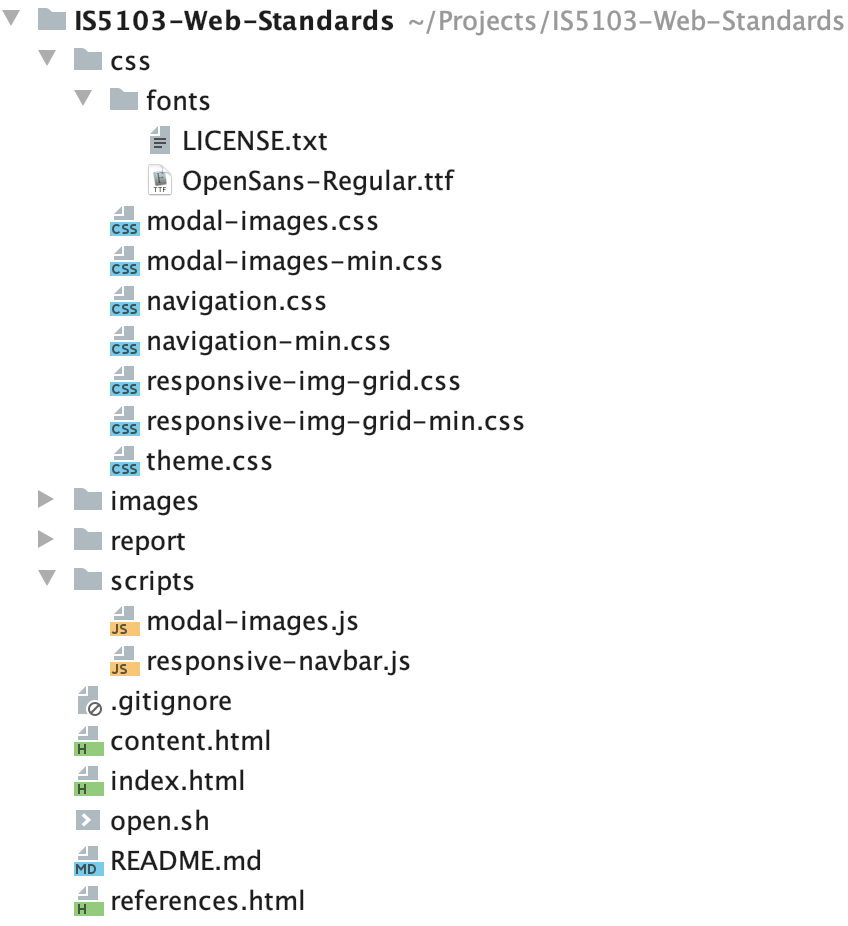
\includegraphics[width=0.5\textwidth]{report/images/root_structure.png}}
\caption{\label{fig:root-structure}A screenshot of the project's root structure depicting the organisation of the website's files.}
\end{figure}

\subsection{Early Styling}
\label{sec:design-content-early-styling}

The structure of the website now completed, some styling to make the overall visual impression more user-friendly and readable could be applied. The first step consisted in adding a \textit{favicon} (which was downloaded from \textit{favicon.cc} \cite{faviconcc}), which is a small image displayed in the web browser's tab next to the website's title \cite{jain2003user}.\\

Next, a single stylesheet was created to write general CSS styles and apply them to the markup. The stylesheet added colours to backgrounds and text, manipulated text sizes, fonts and weights, and tuned the alignment of the displayed elements on the page.\\

The colour scheme used was inspired from the \textit{``Sleek and Futuristic''} theme from \textit{Visme}\footnote{Visme \url{https://visme.co/blog/website-color-schemes/}}, which can be seen in Figure \ref{fig:colour-palette}. To allow the website to be easily changed in the future, variables to represent the different colours of the theme were added at the top of the stylesheets, allowing them to be easily modified in a single place rather than repetitively in the entire code.\\

\begin{figure}[h] 
\centerline{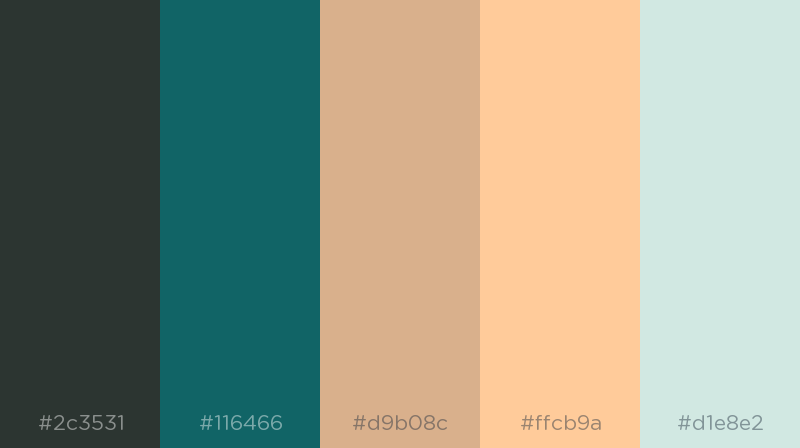
\includegraphics[width=0.7\textwidth]{report/images/colour-palette.png}}
\caption{\label{fig:colour-palette}The colour palette of the \textit{``Sleek and Futuristic''} theme, generated via \textit{coolors.co}.}
\end{figure}

Regarding the font used, \textit{OpenSans-Regular} font was used as it has a \textit{``high readability and friendly appearance. [It] has excellent legibility and its letterforms are incredibly strong with the very extensive font library.''} \cite{open-sans-font}. Additionally, it allowed me to learn where to download fonts, how to import them in the stylesheets and where to store them in the project structure.\\

Icons from the W3.CSS Icons Library \cite{w3-css-icons} were used to make the navbar links and footer more friendly, as seen in Figure \ref{fig:navbar-icons}. From personal experience, a heart is always added in the footer to make the website feel more friendly to the user.

\begin{figure}[h] 
\centerline{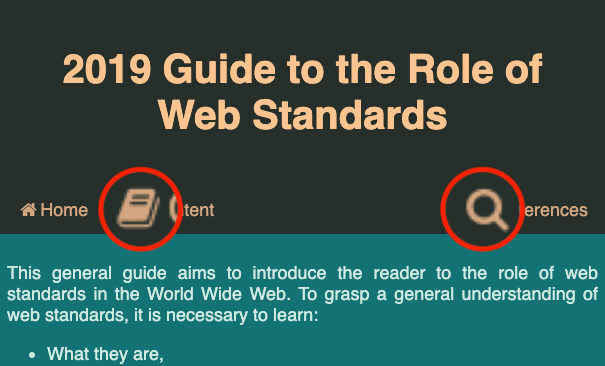
\includegraphics[width=0.7\textwidth]{report/images/navbar-icons.png}}
\caption{\label{fig:navbar-icons}A screenshot of the navbar, with a zoom on the use of icons.}
\end{figure}

During the development of all the aforementioned CSS styles, Chrome's developer tools, which includes a DOM element inspector \cite{chrome-dev-tools}, was used to modify and apply CSS styles live in order to determine the best values for the elements such as font sizes, paddings and margins.\\

To improve the style and readability of the pages, minor HTML elements were added such as thematic breaks \textit{\textless hr\textgreater}, line breaks \textit{\textless br\textgreater} and links to external websites opening in new tabs by using \textit{target=``\_blank''} in the anchor tags \textit{\textless a\textgreater}. Additionally, the footer was modified to stick at the bottom of the page rather than floating up when there is not enough content to fill the page.

\subsection{Advanced Styling}
\label{sec:advanced-styling}

At this stage, the basic website is done and development could have been halted, but a couple of advanced styles, which involved both CSS and JavaScript, were worth being added on top of the existing features.\\

The first improvement consisted in making efficient and elegant use of the home page to clearly separate the six subtopics. This was achieved through the implementation of a grid of images, which revealed the subtopic's title when hovered and routed the user to the corresponding subtopic upon mouse click, as depicted in Figure \ref{fig:grid-images-hover}. 

\begin{figure}[h] 
\centerline{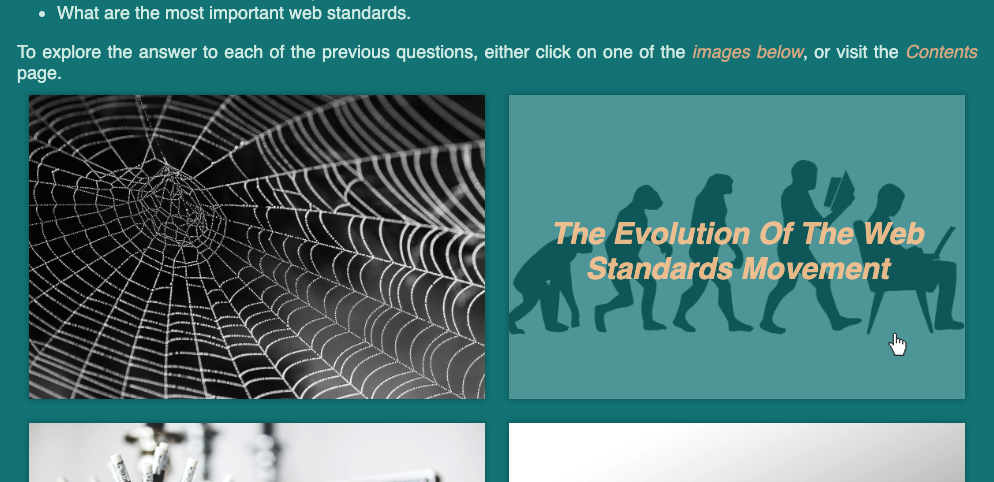
\includegraphics[width=0.8\textwidth]{report/images/grid-images-hover.png}}
\caption{\label{fig:grid-images-hover}A screenshot of the grid of images, with the mouse hovering the right image, triggering the title to appear.}
\end{figure}

A tutorial from Menucool \cite{menucool} was followed to successfully implement this feature, and external code was therefore used. This allowed me to strengthen my understanding of CSS written by other web developers and the ability to understand and modify existing CSS to satisfy the website's requirements. The style handling the grid of images can be found at \textit{``css/modal-images.css''}. The six photos used were provided by Pexels\footnote{Pexels: \url{https://www.pexels.com/photo-license/}.} could be re-used for free.\\

The second improvement targeted the figures used in the \textit{Contents} page. Indeed, it was initially very hard to discern details on the images, especially on mobile devices, without zooming in manually. Therefore, image modals from the W3School \cite{w3s-image-modals} were implemented to allow the user to click on one of the three figures from the \textit{Contents} page to view it scaled up in a fullscreen view with a dark background. Benefits of images modals are further discussed in Section \ref{sec:accessibility}.

\subsection{Responsiveness}
\label{sec:responsiveness}

Most of the style that has been written so far suits large screens (desktop and laptop devices), but it does not suit small screens yet (mobile devices). Therefore, the website had to be made responsive to adapt to any screen size. This was mainly achieved through the use of \textit{media queries}, which act as breakpoints in CSS when applying style by checking the size of the current screen to decide which style to apply to the markup elements \cite{responsive-media-queries}.\\

The first element that needed responsiveness was the navbar. Indeed, on smaller screens, the navbar links on the left and the right did not align properly, which visually appeared very poor. The solution was to collapse all the links except the home link and to add an extra button (link with only an icon) that reveal the hidden links when pressed, as seen in Figure \ref{fig:mobile-navbar}. The W3School tutorial on how to make responsive navbars \cite{responsive-navbar} was followed to implement this feature.

\begin{figure}[h] 
\centerline{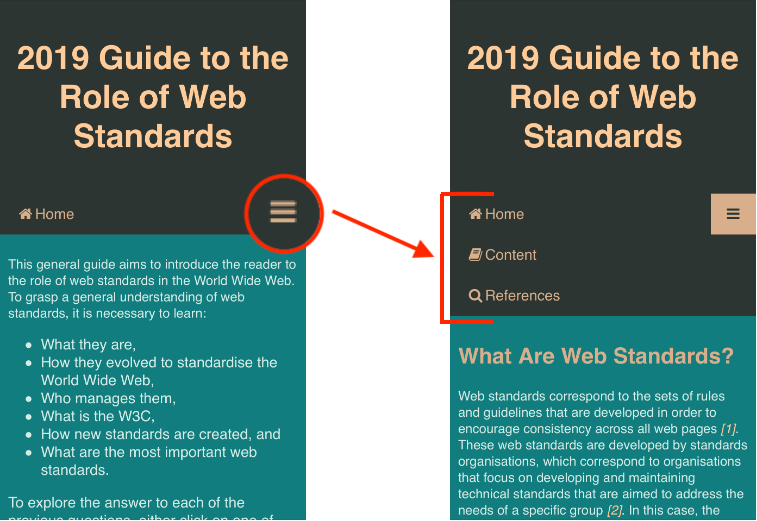
\includegraphics[width=0.8\textwidth]{report/images/mobile-navbar.png}}
\caption{\label{fig:mobile-navbar}A screenshot of the navbar on a small mobile screen. To the left, the links are collapsed and revealed upon a button press, which expands the other links, as seen on the right.}
\end{figure}

Finally, multiple elements required a responsive design when switching to small screens. These included:
\begin{itemize}
    \item In the grid of images on the \textit{Home} page, display only a single cell on small screens and two on large screens.
    \item Regarding text, make the size smaller and alignment on the left on mobile devices to improve readability.
\end{itemize}

\subsection{Optimisation}

Lastly, a few improvements were carried out maximise the loading speed of the website. Logically, large file sizes are a major enemy when it comes to loading a page swiftly. Therefore, all PNG images were converted to a JPEG format, before being compressed online\footnote{CompressJPEG was used to compress the images: \url{https://compressjpeg.com/}.} to reduce their file size. This resulted in images originally weighing between 1.5Mb-2Mb to weighing less than 500Kb after the compressions.\\

Furthermore, it important to note that importing stylesheets in the HTML \textit{\textless head\textgreater} can be a costly operation in terms of time, especially when there are many stylesheets. As a result, the CSS styles were separated into only four stylesheets, and minified\footnote{The CSS stylesheets were minified through CSSMinifier: \url{https://cssminifier.com/}.} for quicker imports. Additionally, online stylesheets such as the Font Awesome stylesheet \cite{w3-css-icons} were not downloaded and locally accessed but rather imported via CDN\footnote{Content Delivery Networks} for higher performance \cite{dilley2002globally}.

% ---------------------------------------------------------------------------

\section{Accessibility}
\label{sec:accessibility}

Multiple features were progressively added to the website to favour accessibility to all users. The first one is the colour scheme mentioned in Section \ref{sec:design-content-early-styling}, which favours high-contrast between text and background. The Chrome element inspector developer tool was used to view the contrast between text colour and background colour, which, according to the tool, was acceptable across the entire website. The image modals mentioned in Section \ref{sec:advanced-styling} also help users on small screens and visually impaired users as it allows the figures to be seen in fullscreen with a dark background. Screenshots of the contrast results can be found in Appendix \ref{sec:appendix-accessibility-results-contrast}.\\

Keyboard accessibility was also taken into account for disabled users who cannot use their computer mouse. When tabbing across the website, the active link is highlighted with a thick bright red border (see Appendix \ref{sec:appendix-accessibility-results-keyboard}). This includes navbar links, the grid images, and any link pointing to other sections, references or external websites. Additionally, the red border also appears when clicking on those links to help visually impaired and colour-blind users know that they clicked the link correctly. This was achieved by styling selected anchor tags \textit{\textless a\textgreater} using the CSS \textit{:focus} pseudo-class \cite{css-focus}.

% ---------------------------------------------------------------------------

\section{Testing and Evaluation}
\label{sec:testing-evaluation}

\subsection{Code Testing}

To test the website, every interactive element was clicked on every page of the website. This included clicking on:
\begin{itemize}
    \item each navbar link \textbf{from every page}, in case a link works on one page but not another.
    \item on each of the six grid images and making sure they linked to the correct subtopic.
    \item on each link to another section or figure.
    \item on each citation e.g. \textit{[6]}, to make sure it redirected the user to the \textit{References} page.
    \item on each external link in the \textit{References} page to make sure it opened to the correct link in a new tab.
\end{itemize}

\subsection{User Evaluation Feedback}

Ten users were asked to explore the website before filling out a form that asked them questions about the website's readability, accessibility, responsiveness and style, the device used and the potential improvements they would like to see. The form was provided via Google Forms and can be found in Appendix \ref{sec:appendix-user-evaluation-form}. The full results to each question of the form can be found in Appendix \ref{sec:appendix-user-evaluation-results}.\\

The evaluation revealed that all users found the website readable, mainly thanks to the colours. However, a few users complained about the colours being \textit{``dark''}, which was taken into account by increasing the brightness on the blue and beige colours from Figure \ref{fig:colour-palette} (which was an easy operation thanks to the colours being declared in the root of each stylesheet). The users also found the web site to be responsive to smaller screens, saying that it ``adapted'' well to mobile devices. This is important since 80\% of the users tested the website on a mobile device.\\

Regarding accessibility, 40\% of users believed the website would be suitable to visually impaired reader, while 60\% answered \textit{``maybe''}. This depicts that more features could have been implemented to achieve higher accessibility. One feature that was attempted, but ended up taking too long, was adding a button on the navbar that allowed the user to toggle between different colour theme. The goal was to have the current theme switch to a basic white background / black text theme with bigger text sizes in order to facilitate the reading experience.

\subsection{Code Validation}

The HTML and CSS were regularly tested across development using the official online code checkers provided by the W3C. The three HTML files were uploaded to the W3C Markup Validation Service\footnote{W3C Markup Validation Service: \url{https://validator.w3.org}.}, and all three of them passed with (full reports an be found in Appendix \ref{sec:appendix-validation-reports}):

\begin{itemize}
    \item \textit{index.html}: 0 warnings, 0 errors.
    \item \textit{content.html}: 0 warnings, 0 errors.
    \item \textit{references.html}: 0 warnings, 0 errors.
\end{itemize}

\subsection{Responsiveness Evaluation}

The website was first tested on different browsers, including Chrome, Safari, Mozilla Firefox and Edge. All of the website's pages were displayed identically throughout all web browsers.\\

Next, the website was tested on different devices, namely desktop and mobile devices. All of the styling detailed in Section \ref{sec:responsiveness} was correctly applied to the mobile device. A full comparison of desktop and mobile versions of the website can be found in Appendix \ref{sec:appendix-device-responsiveness}. A couple of improvements that could be carried out include the breaking of long links on the \textit{References} page and adapting the grid of images for mobile devices according to the user evaluation as a user noticed that mobile devices do not display the title of the section when hovering over an image.\\

To ensure that the styling was applied at the right moment, an experience was carried out where the web browser's window was gradually shrunk on its horizontal axis, causing the elements on the page to start squeezing before the CSS for small screens began being applied on various elements such as collapsing the navbar or display a single image on the grid of images.

\section{Website Hosting}
\label{sec:website-hosting}

The website is hosted on a nginx web server provided by the University of St Andrews. It can be visited at the following URL: \url{https://agj6.host.cs.st-andrews.ac.uk/}.

\section{Conclusions}
\label{sec:conclusions}

Making a website consisting only of HTML markup and CSS is to a certain extent easy. The real difficulty lies with making a website:
\begin{itemize}
    \item \textit{responsive} to multiple screen sizes, including less used devices such as tablets or televisions.
    \item \textit{accessible} to everyone, taking as many disabilities into consideration.
    \item \textit{well-structured} and organised.
    \item easily \textit{scalable}, allowing for maintenance and change without unnecessary overheads.
    \item \textit{quick}, not wasting time loading.
    \item \textit{compliant} to web standards.
\end{itemize}

% ---------------------------------------------------------------------------

\begin{appendices}

\newpage
\bibliographystyle{unsrt}
\bibliography{bibliography}

\clearpage
\section{Evidence of Prior Planning}

\subsection{Research Essay}
\label{sec:appendix-prior-planning-research-essay}

\begin{figure}[h] 
\centerline{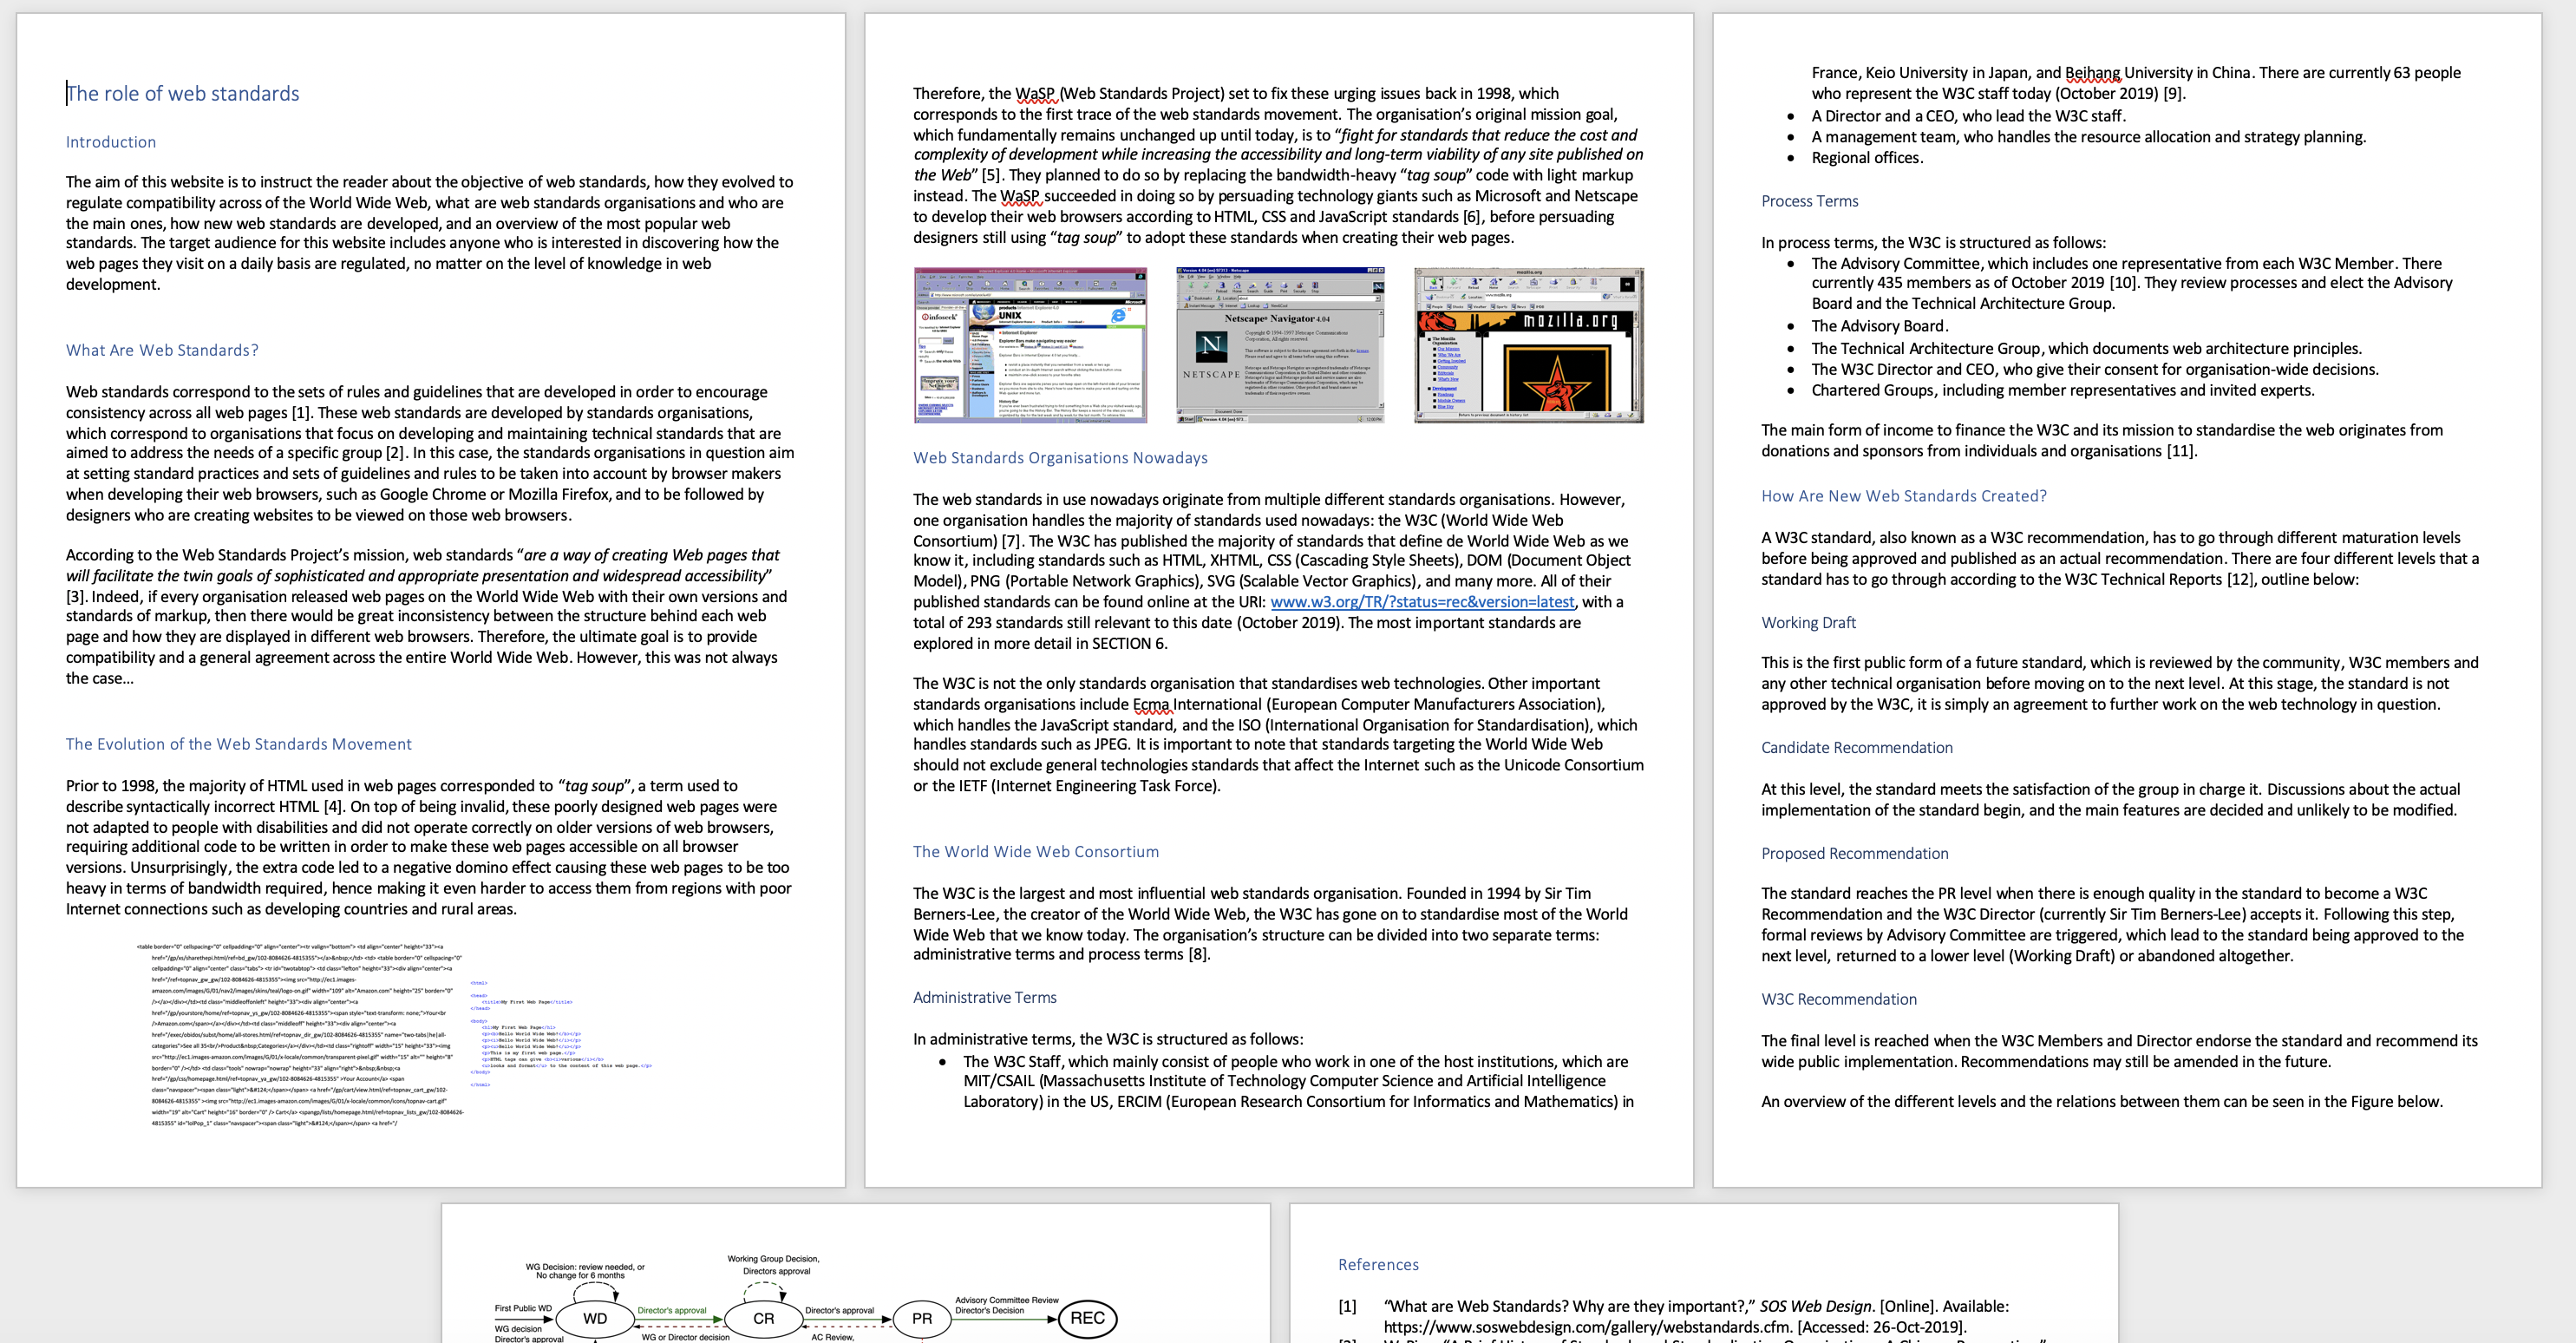
\includegraphics[width=1.1\textwidth]{report/images/prior-planning-research.png}}
\caption{\label{fig:prior-planning-research}A screenshot of the research carried out in a Word document.}
\end{figure}

\subsection{Initial Draft}
\label{sec:appendix-prior-initial-draft}

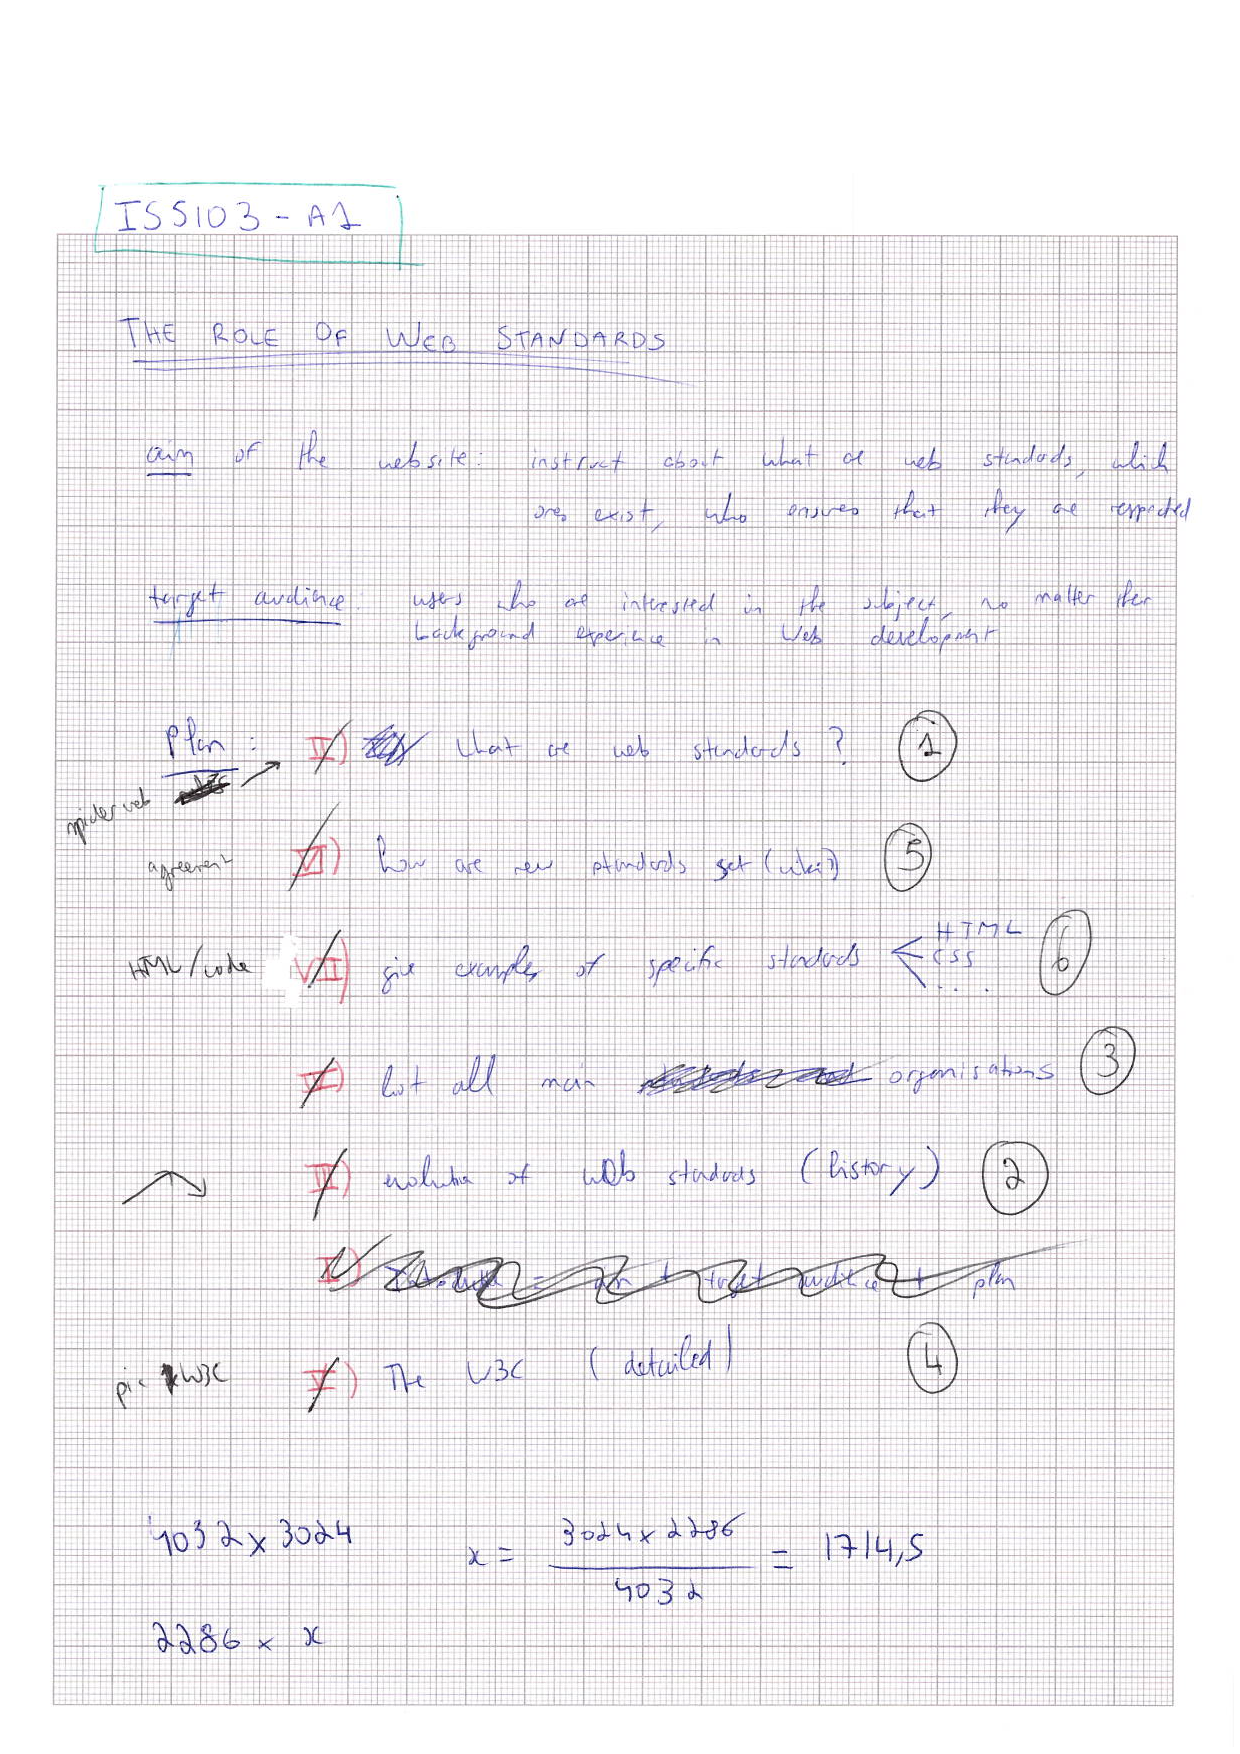
\includepdf[pages={1},pagecommand={},scale=0.9]{report/images/prior-planning.pdf}

\clearpage
\section{Accessibility Results}
\label{sec:appendix-accessibility-results}

\subsection{Contrast Results}
\label{sec:appendix-accessibility-results-contrast}

\begin{figure}[h] 
\centerline{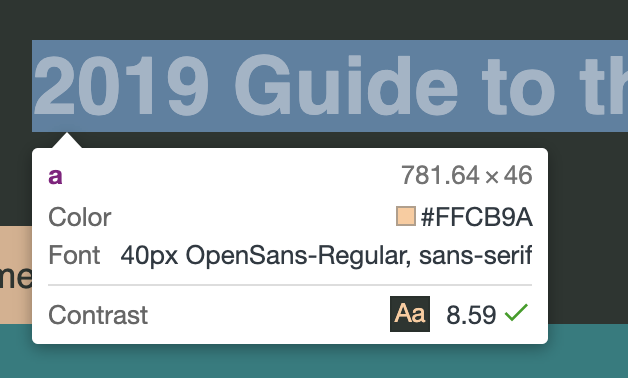
\includegraphics[width=0.7\textwidth]{report/images/accessibility-contrast-header.png}}
\caption{\label{fig:accessibility-contrast-header}Screenshot of the contrast result of the Chrome developer tool element inspector for the header's text.}
\end{figure}

\begin{figure}[h] 
\centerline{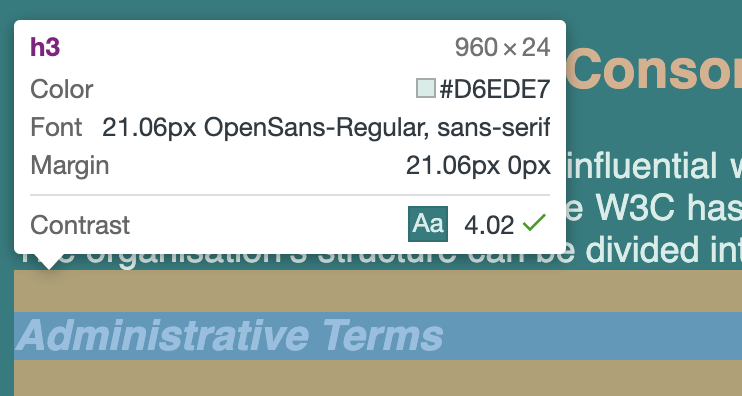
\includegraphics[width=0.8\textwidth]{report/images/accessibility-contrast-text.png}}
\caption{\label{fig:accessibility-contrast-text}Screenshot of the contrast result of the Chrome developer tool element inspector for the main content's text.}
\end{figure}

\begin{figure}[ht] 
\centerline{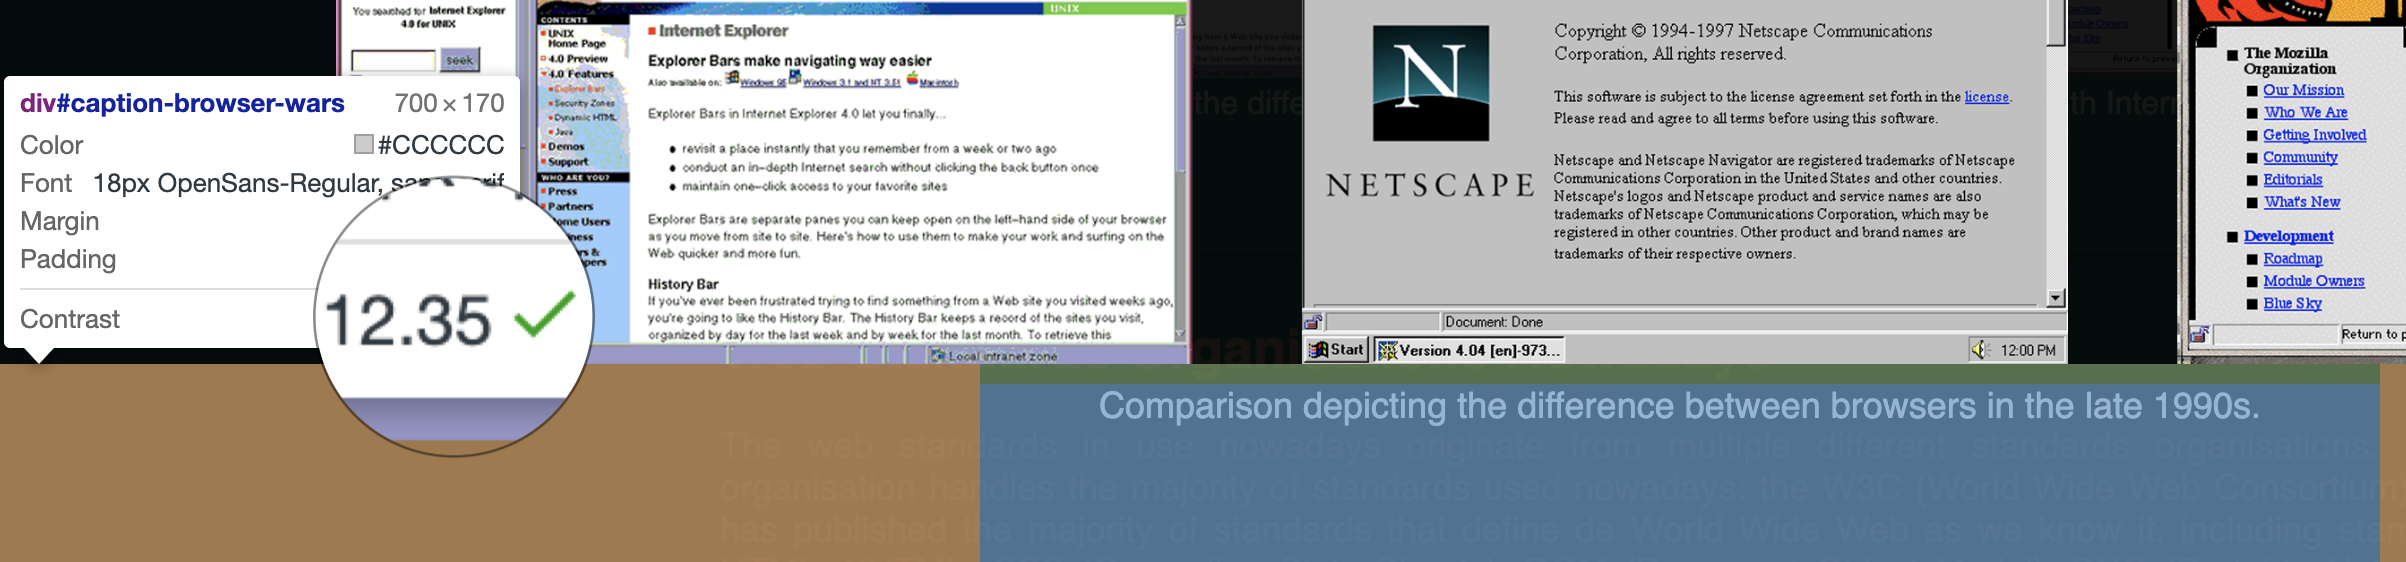
\includegraphics[width=\textwidth]{report/images/accessibility-contrast-modal.png}}
\caption{\label{fig:accessibility-contrast-modal}Screenshot of the contrast result of the Chrome developer tool element inspector for one of the figure's modal in fullscreen.}
\end{figure}

\subsection{Keyboard Accessibility Screenshot}
\label{sec:appendix-accessibility-results-keyboard}

\begin{figure}[h] 
\centerline{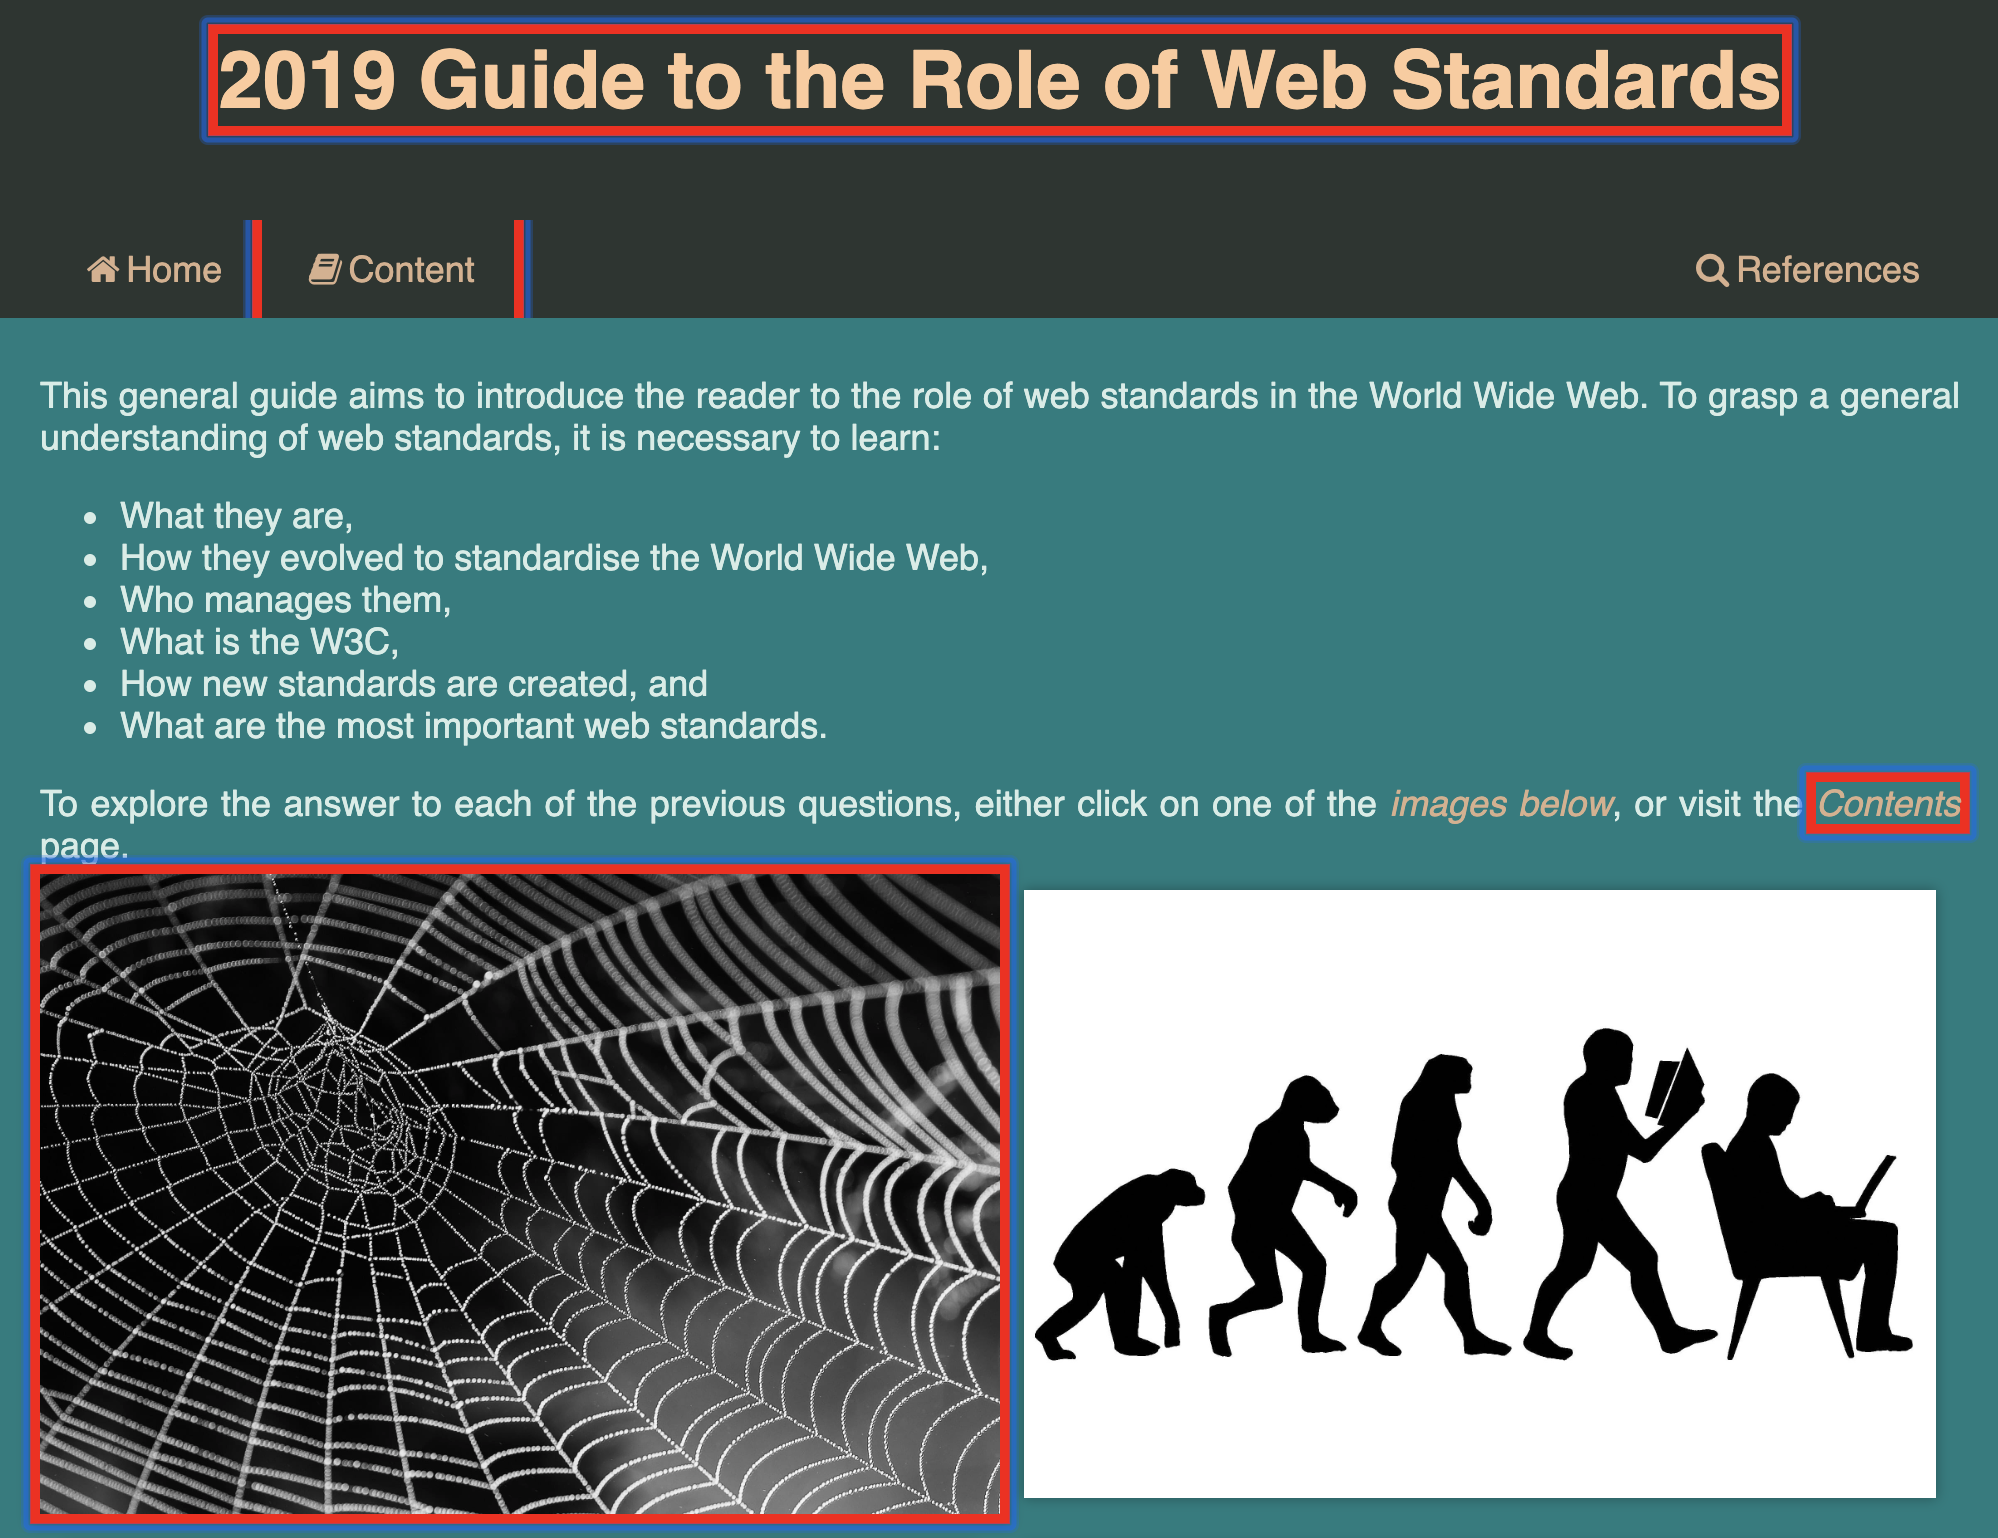
\includegraphics[width=\textwidth]{report/images/border-focus.png}}
\caption{\label{fig:border-focus}Screenshot of the \textit{Home} page with multiple links set on \textit{:focus} to illustrate the bright red border surrounding each element when navigating through the page using either the \textit{tab} key or when clicking one of the links.}
\end{figure}

\clearpage
\section{User Evaluation}

\subsection{User Evaluation Form}
\label{sec:appendix-user-evaluation-form}

The user evaluation is powered by Google Forms and is available online at \url{https://forms.gle/FHY6LDmY65GQa33s8}.

\paragraph{Description} This is a user evaluation of the website made for Assignment 1 of IS5103 Web Technologies module. The website aims to introduce the reader to the role of web standards.\\

Note: The data retrieved from this user evaluation will be anonymously compared to other results. By submitting this form, you give consent for your data to be evaluated and used in the report. You may withdraw from the user evaluation at any time.

\paragraph{Visit the website} \url{https://agj6.host.cs.st-andrews.ac.uk/index.html}

\paragraph{Questions}

\begin{itemize}
    \item How readable did you find the website?
    \begin{itemize}
        \item Answer: 5-point linear scale (as shown in Figure \ref{fig:linear-scale}).
    \end{itemize}
\end{itemize}

\begin{figure}[h] 
\centerline{
\includegraphics[width=0.75\textwidth]{report/images/linear_scale.png}}
\caption{\label{fig:linear-scale}Illustration of the 5-point linear scale used to record an answer, ranging from 1 to 5.}
\end{figure}

\begin{itemize}
    \item What are the main aspects/elements that make the website readable e.g. colours, spacing, fonts, etc.
    \begin{itemize}
        \item Answer: short paragraph.
    \end{itemize}
\end{itemize}

\begin{itemize}
    \item Do you think this website would be suitable to visually impaired readers?
    \begin{itemize}
        \item Answer: multiple choice question:
        \begin{itemize}
            \item Yes
            \item No
            \item Maybe
        \end{itemize}
    \end{itemize}
\end{itemize}

\begin{itemize}
    \item What are the main aspects/elements that make the website accessible to everyone?
    \begin{itemize}
        \item Answer: short paragraph.
    \end{itemize}
\end{itemize}

\begin{itemize}
    \item What would you change about the website to improve it?
    \begin{itemize}
        \item Answer: short paragraph.
    \end{itemize}
\end{itemize}

\begin{itemize}
    \item Have you tested the website on desktop or mobile?
    \begin{itemize}
        \item Answer: multiple choice question:
        \begin{itemize}
            \item Yes
            \item No
        \end{itemize}
    \end{itemize}
\end{itemize}

\begin{itemize}
    \item If you tested the website on mobile, how would you rate the responsiveness of the website (how well did it scale from large screens to small screens)?
    \begin{itemize}
        \item Answer: 5-point linear scale (as shown in Figure \ref{fig:linear-scale}).
    \end{itemize}
\end{itemize}

\subsection{User Evaluation Results}
\label{sec:appendix-user-evaluation-results}

The user evaluation was carried out with a total of 10 users. Their answers to each question are listed below.

\begin{itemize}
    \item How readable did you find the website?
\end{itemize}

\begin{figure}[h] 
\centerline{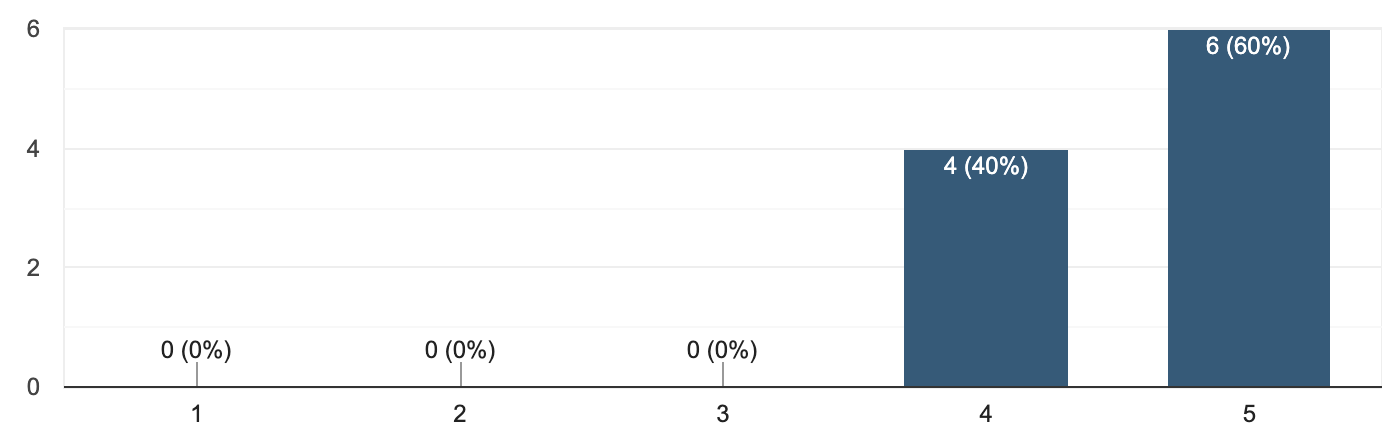
\includegraphics[width=0.9\textwidth]{report/images/user-survey-site-readability.png}}
{\label{fig:user-survey-site-readability}}
\end{figure}

\begin{itemize}
    \item What are the main aspects/elements that make the website readable e.g. colours, spacing, fonts, etc.
    \begin{itemize}
        \item 	participant 1: 	colours very appeasing 
    \item 	participant 2: 	colour scheme, home page images are nice, can click on images to make them bigger
    \item 	participant 3: 	layout and colours
    \item 	participant 4: 	Looks good overall, visually pleasing
    \item 	participant 5: 	The use of colours 
    \item 	participant 6: 	Large text, vibrant colours, adapting to device reading on
    \item 	participant 7: 	The colours used (good contrast), the clear structure
    \item 	participant 8: 	The balance between text and font is perfect!
    \item 	participant 9: 	Colours
    \item 	participant 10: 	font and structure of webpage
    \end{itemize}
\end{itemize}

\begin{itemize}
    \item Do you think this website would be suitable to visually impaired readers?
\end{itemize}

\begin{figure}[h] 
\centerline{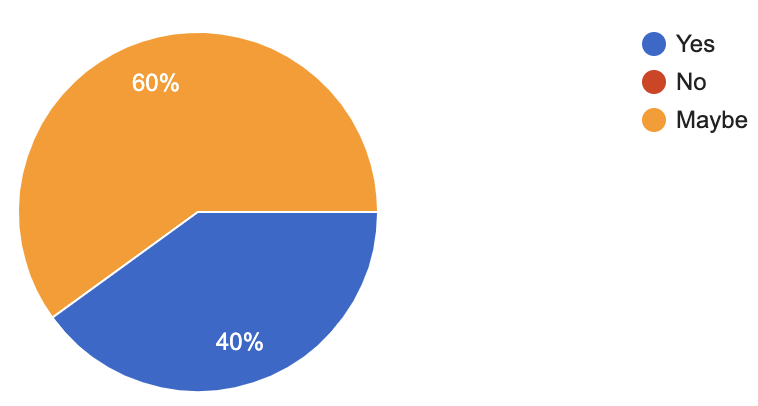
\includegraphics[width=0.75\textwidth]{report/images/user-survey-visually-impaired.png}}
{\label{fig:user-survey-visually-impaired}}
\end{figure}

\begin{itemize}
    \item What are the main aspects/elements that make the website accessible to everyone?
    \begin{itemize}
        \item 	participant 1: 	simple site, to the point
        \item 	participant 2: 	red boxes when clicking
        \item 	participant 3: 	easy access
        \item 	participant 4: 	Clear separation of sections
        \item 	participant 5: 	The font size was adequate 
        \item 	participant 6: 	Pictures, adapting to different devices
        \item 	participant 7: 	Simple manoeuvring, interactive set-up
        \item 	participant 8: 	Subtle colours, readable font, and clear copy.
        \item 	participant 9: 	Fonts
        \item 	participant 10: pictures
    \end{itemize}
\end{itemize}

\begin{itemize}
    \item What would you change about the website to improve it?
    \begin{itemize}
        \item 	participant 1: 	make it fill the screen
        \item 	participant 2: 	add more colour options
        \item 	participant 3: 	nothing
        \item 	participant 4: 	Less dark background, dynamic url on contents page when scrolling down
        \item 	participant 5: 	Change the way the pictures are all the end, maybe move them around a little bit 
        \item 	participant 6: 	nothing
        \item 	participant 7: 	Maybe a little bigger font or more room between the lines
        \item 	participant 8: 	Nothing
        \item 	participant 9: 	nothing
        \item 	participant 10: 	on the phone, you are unable to see where each picture directs you. Also make it a bit prettier (the colours are quite dull)
    \end{itemize}
\end{itemize}

\begin{itemize}
    \item Have you tested the website on desktop or mobile?
\end{itemize}

\begin{figure}[h] 
\centerline{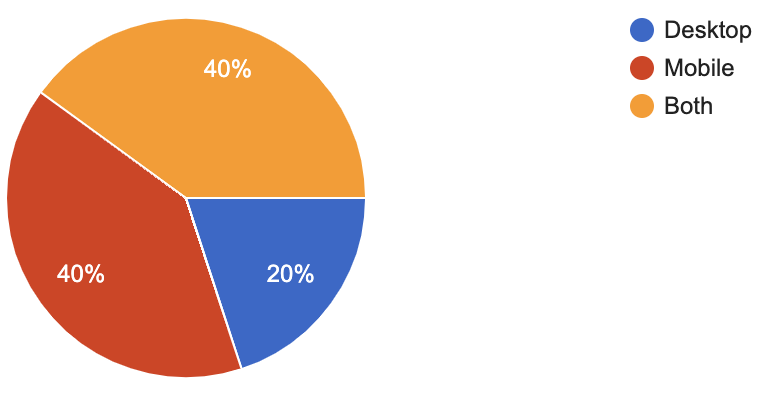
\includegraphics[width=0.75\textwidth]{report/images/user-survey-device.png}}
{\label{fig:user-survey-device}}
\end{figure}

\begin{itemize}
    \item If you tested the website on mobile, how would you rate the responsiveness of the website (how well did it scale from large screens to small screens)?
\end{itemize}

\begin{figure}[h] 
\centerline{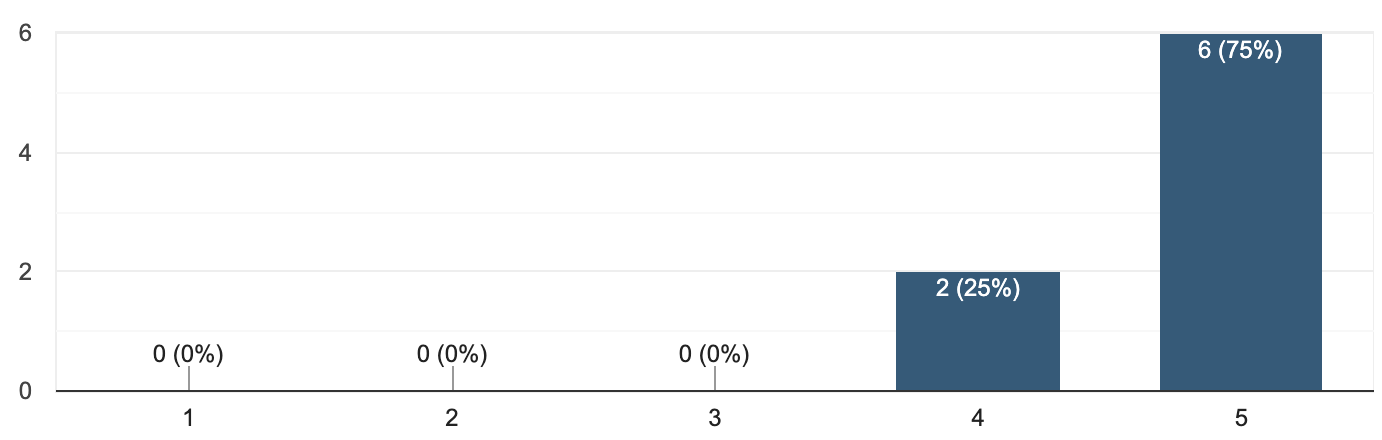
\includegraphics[width=0.9\textwidth]{report/images/user-survey-responsiveness.png}}
{\label{fig:user-survey-responsiveness}}
\end{figure}

\clearpage
\section{HTML Validation Reports}
\label{sec:appendix-validation-reports}

\begin{figure}[h] 
\centerline{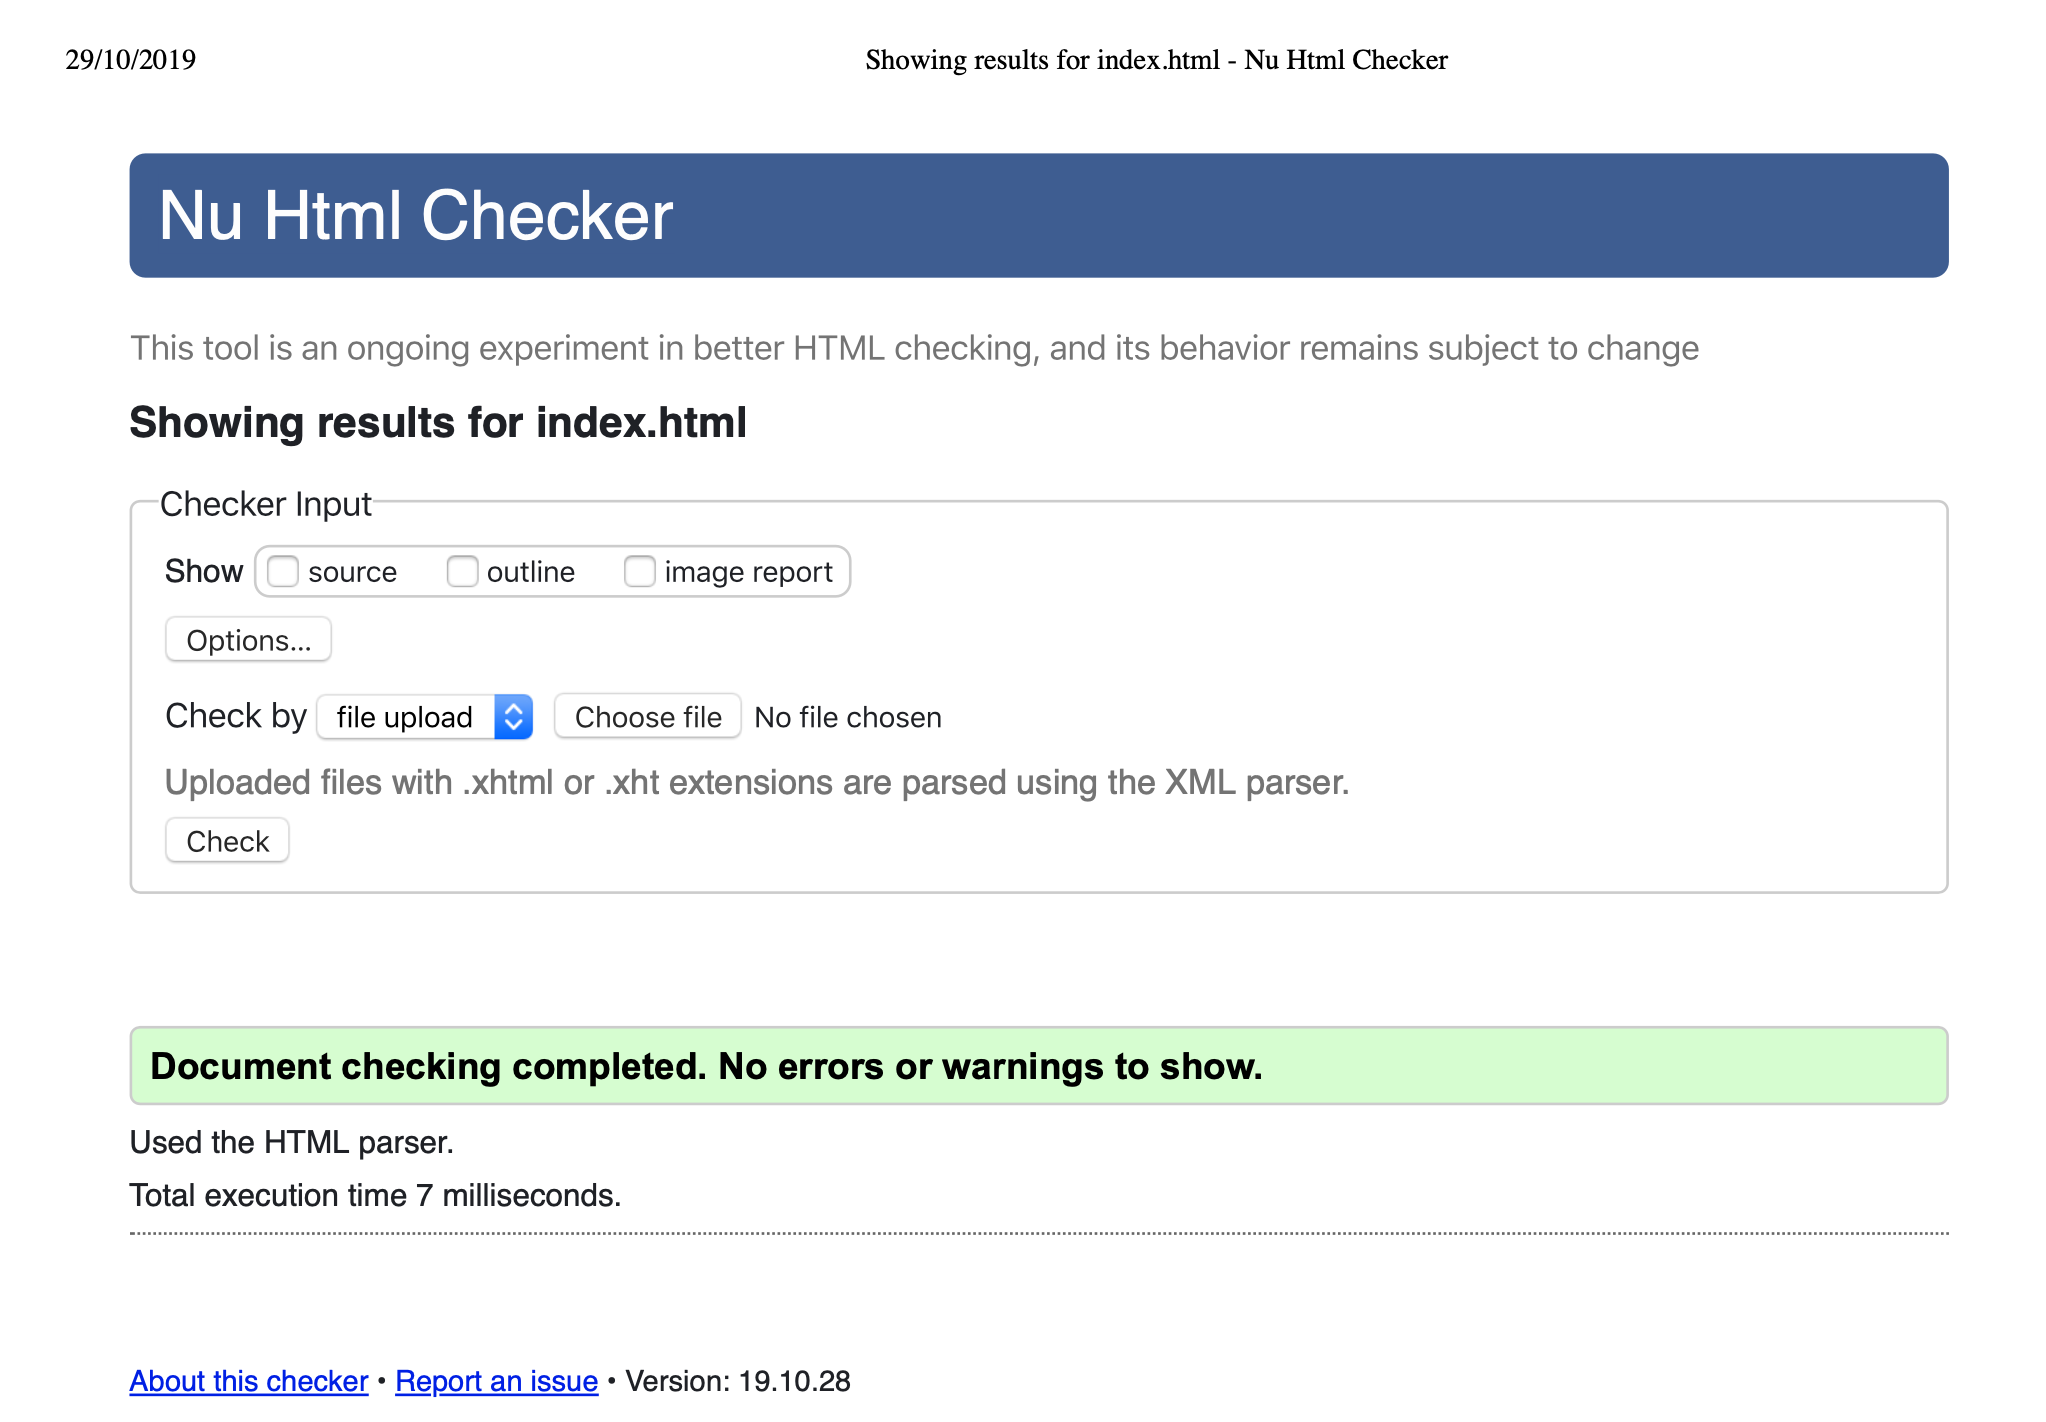
\includegraphics[width=0.8\textwidth]{report/images/validation-index.png}}
\caption{\label{fig:validation-index}Validation of \textit{index.html} file.}
\end{figure}

\begin{figure}[h] 
\centerline{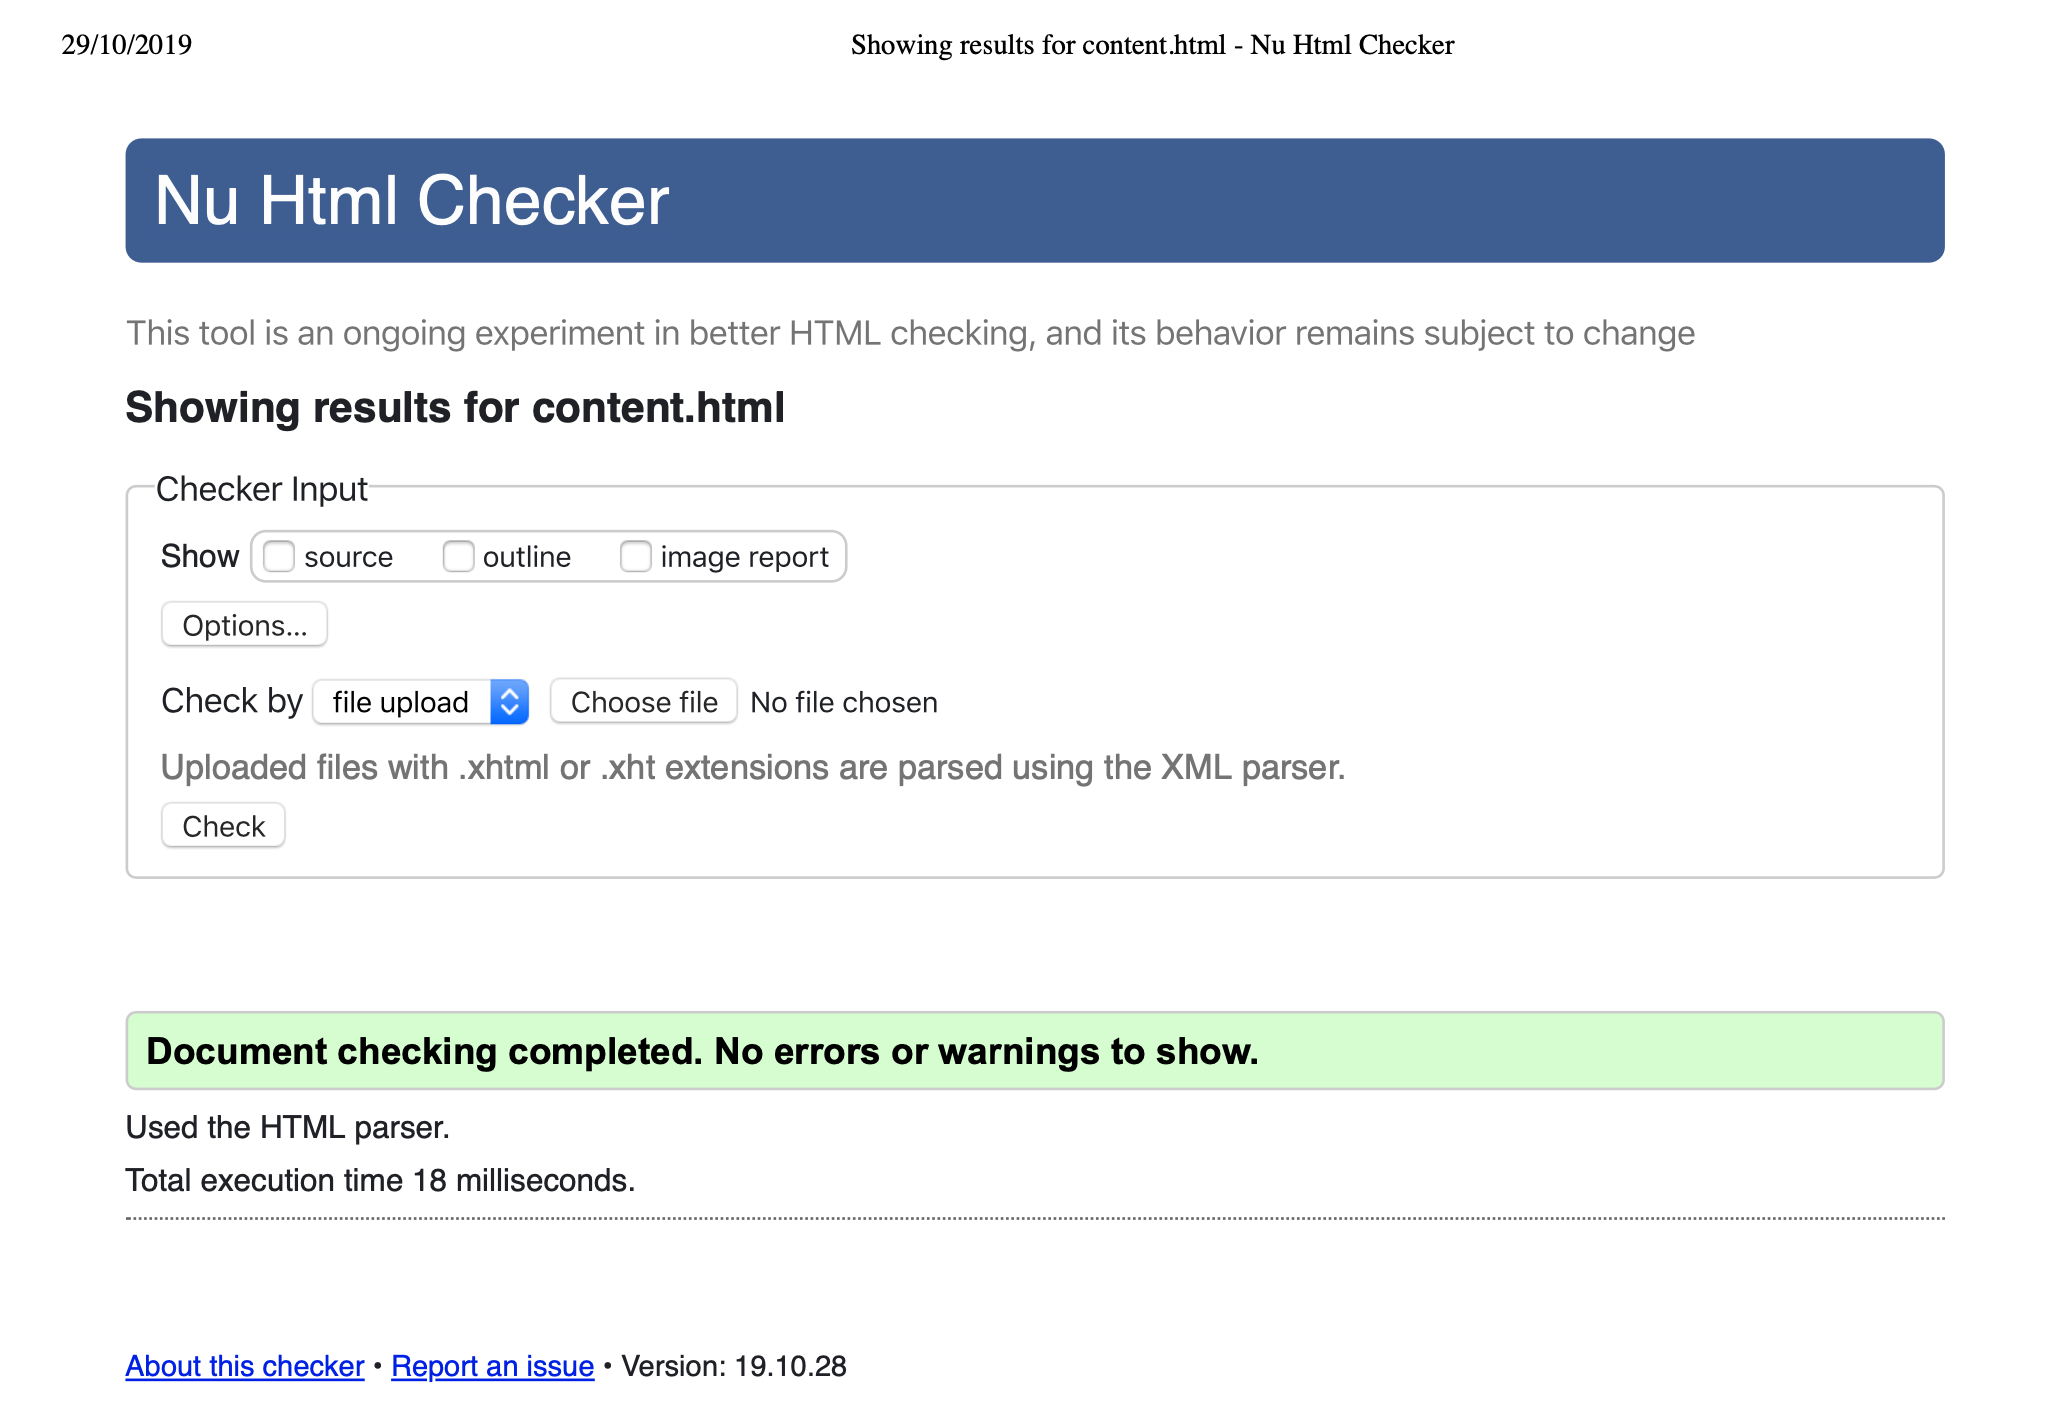
\includegraphics[width=0.8\textwidth]{report/images/validation-content.png}}
\caption{\label{fig:validation-content.png}Validation of \textit{content.html} file.}
\end{figure}

\begin{figure}[h] 
\centerline{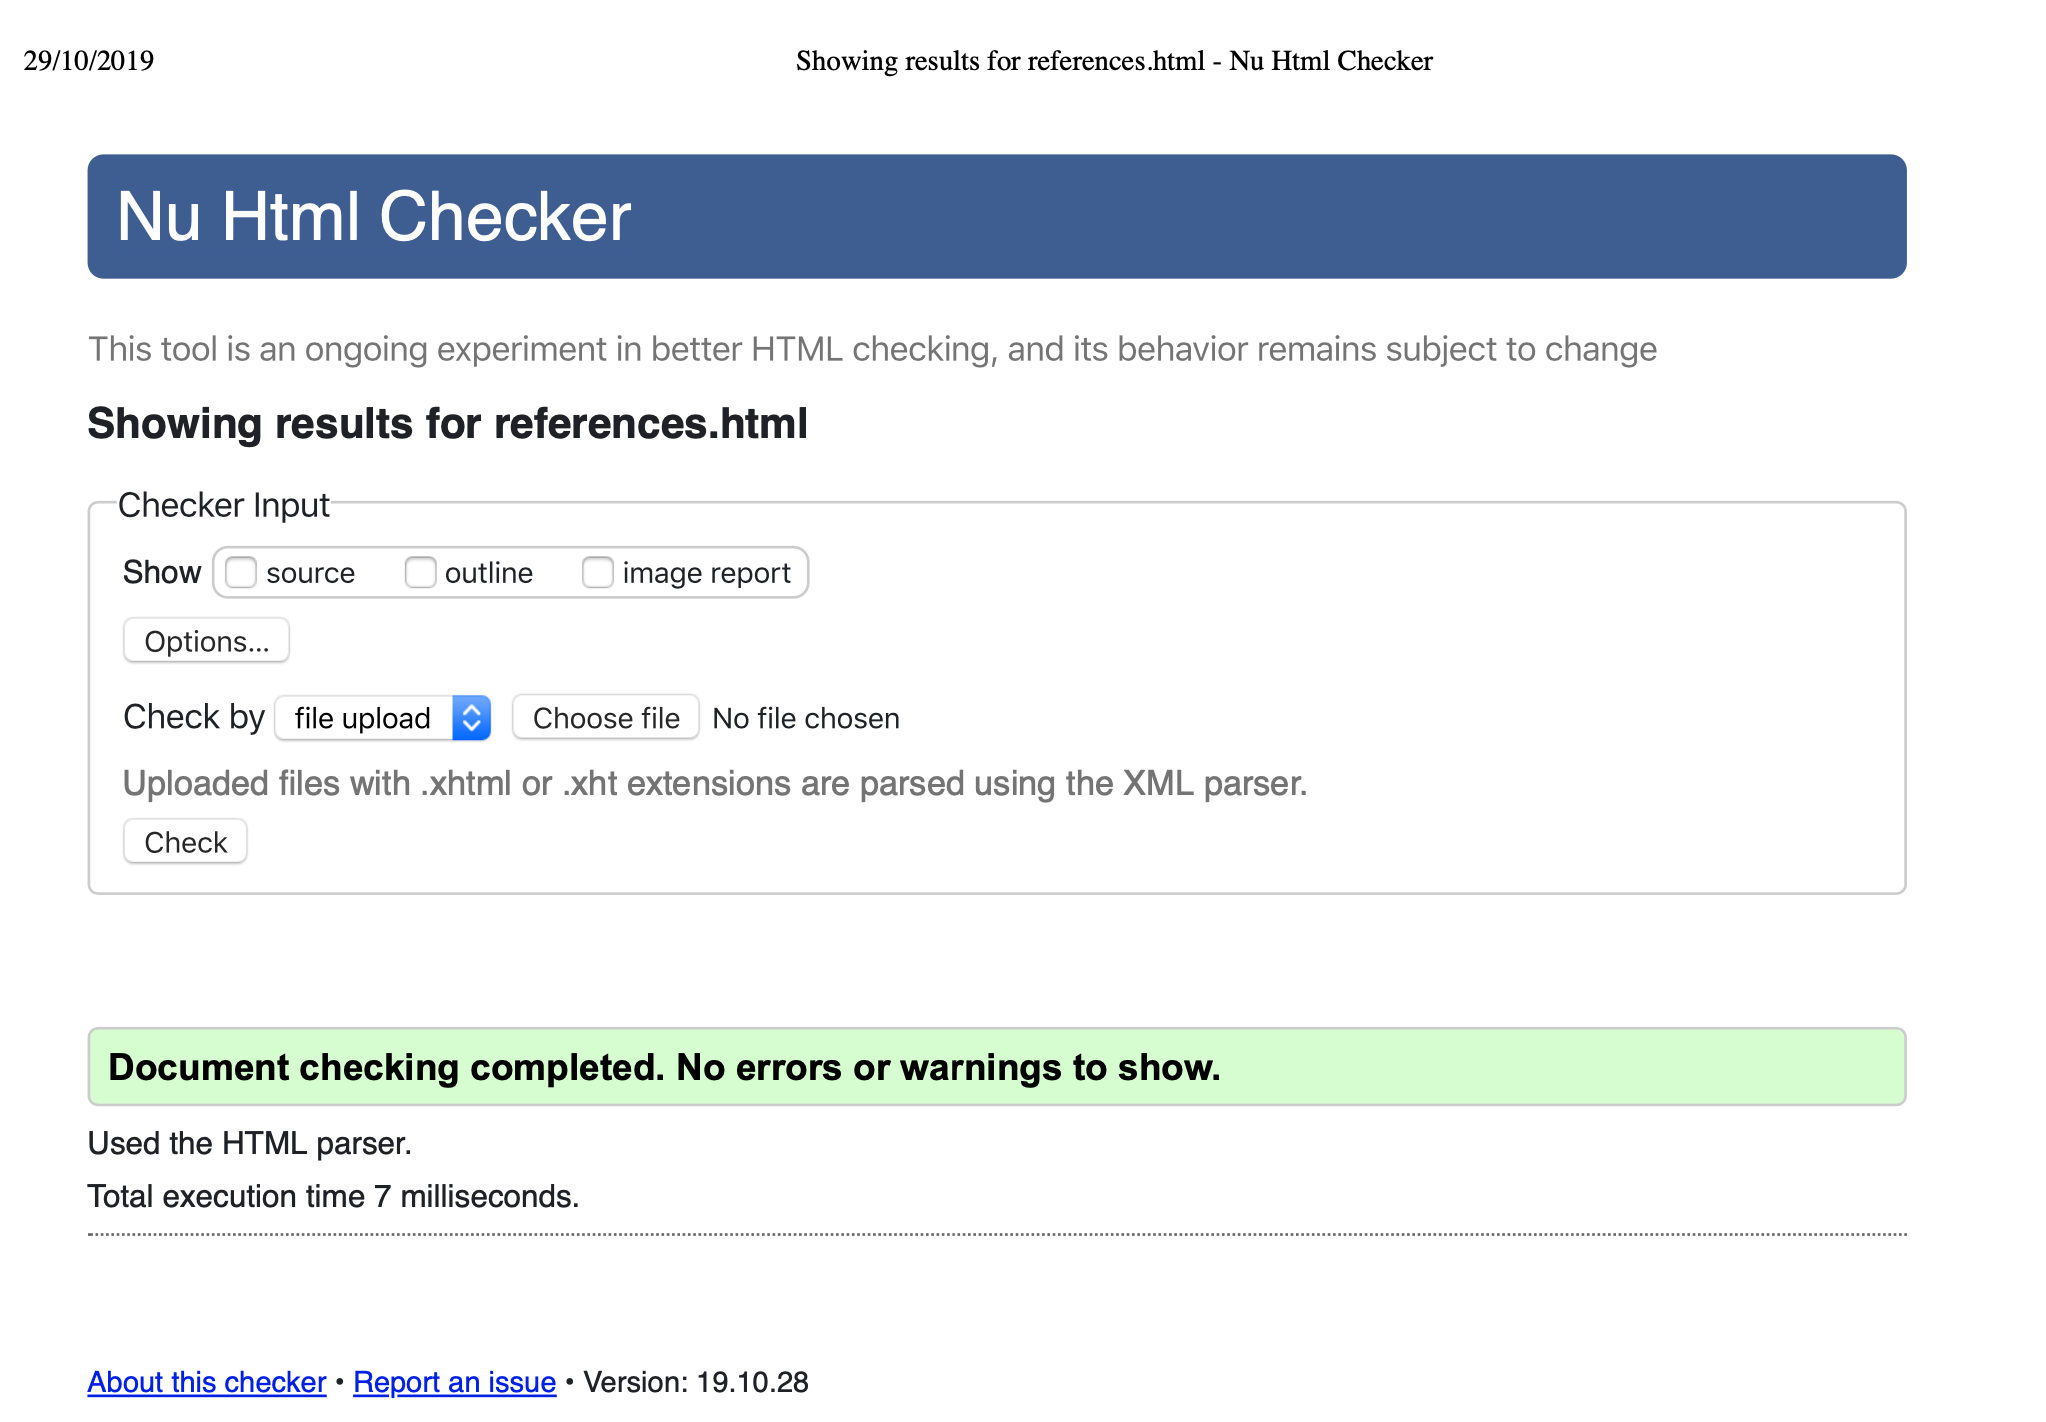
\includegraphics[width=0.8\textwidth]{report/images/validation-references.png}}
\caption{\label{fig:validation-references.png}Validation of \textit{references.html} file.}
\end{figure}

\clearpage
\section{Device Responsiveness}
\label{sec:appendix-device-responsiveness}

\begin{figure}[h] 
\centerline{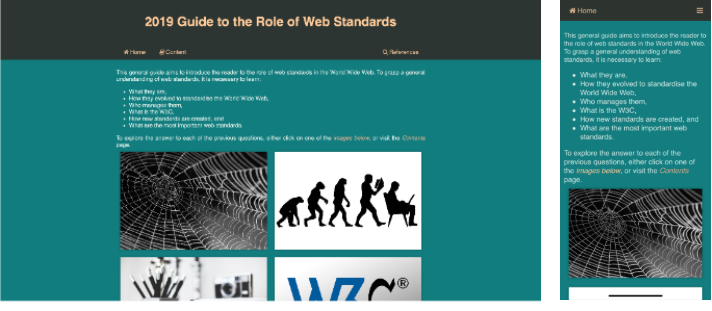
\includegraphics[width=\textwidth]{report/images/comparison-index.png}}
\caption{\label{fig:comparison-index}Comparison of desktop (left) and mobile (right) views of the \textit{Home} page.}
\end{figure}

\begin{figure}[h] 
\centerline{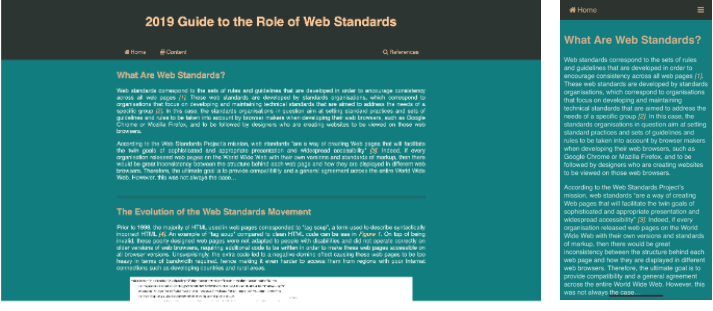
\includegraphics[width=\textwidth]{report/images/comparison-content-top.png}}
\caption{\label{fig:comparison-content-top}Comparison of desktop (left) and mobile (right) views of the \textit{Content} page.}
\end{figure}

\begin{figure}[h] 
\centerline{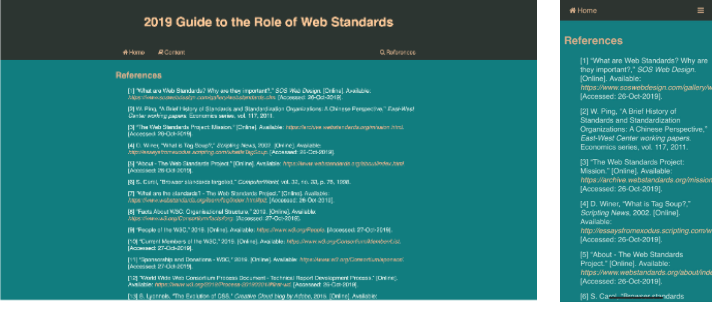
\includegraphics[width=\textwidth]{report/images/comparison-references.png}}
\caption{\label{fig:comparison-references}Comparison of desktop (left) and mobile (right) views of the \textit{References} page.}
\end{figure}

\end{appendices}
\end{document}